% !TEX root = ../Dokumentation.tex
\subsection{Bilderzeugung}
\textbf{Funktionsbeschrieb}\\[0.2cm]
Die Bilderzeugung stellt die Schnittstelle zur Kamera sicher und speichert die erzeugten Bilder fortlaufend in einer von OpenCV zu Verfügung gestellten Datenstruktur. Dabei wird den übrigen Prozessen jeweils nur das aktuellste Bild der Kamera zur Verfügung gestellt.\\
Als Kamera kommt die Raspberry Pi CAM zum Einsatz (Abbildung \ref{fig:camera}), die über eine MIPI Schnittstelle direkt an den Minicomputer angeschlossen und kostengünstig erworben werden kann. Das Bildformat lässt sich über den Open Source Treiber einstellen, was zu einer Performanceverbesserung beiträgt. Der Winkel von 53° ist etwas knapp, daher wird die Kamera drehbar auf dem Fahrzeug montiert. Diese Vorrichtung soll für die Kurvenfahrt sowie den Rechtsvortritt genutzt werden. Der Neigungswinkel der Kamera lässt sich ebenfalls einstellen, um die benötigte Flexibiltät der Sichtposition der Kamera sicherzustellen.
\begin{figure}[H]
\centering
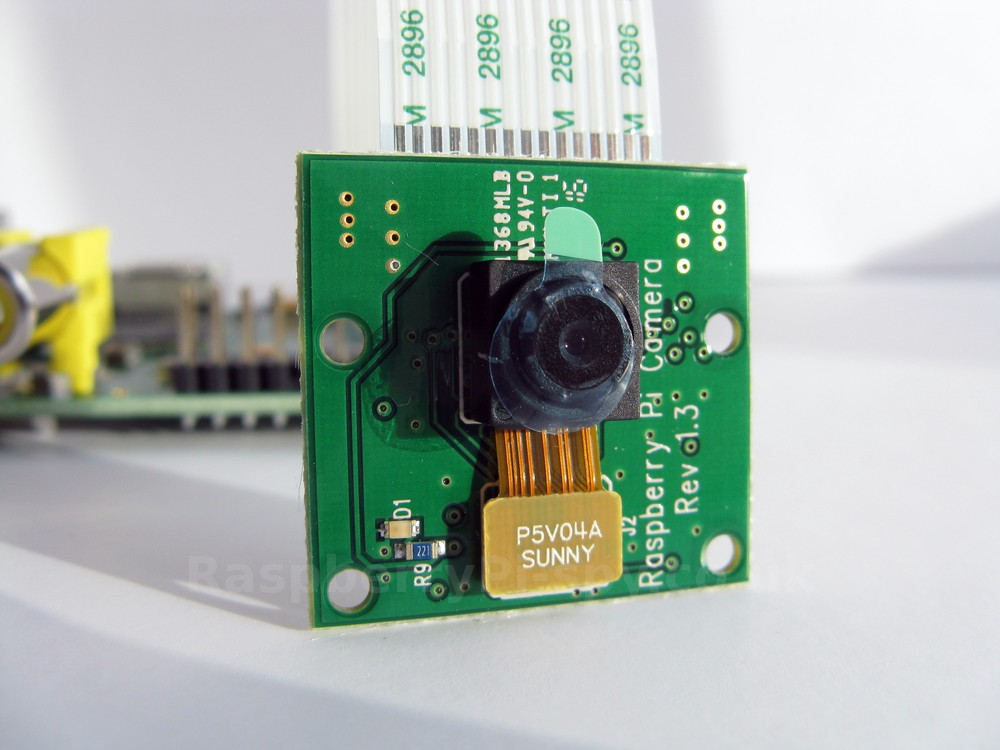
\includegraphics[width=0.6\textwidth]{03_Loesungskonzept/pictures/raspberry-pi-camera-module.jpg}
\caption{Raspberry Pi Kameramudul}
\label{fig:camera}
\end{figure}
\textbf{Komponentenbeschrieb}\\[0.2cm]
Die Bilderzeugung ist ein eigener als Thread realisierter Subprozess und liefert über die Methode \code{GetImage()} den Pointer auf das Bild zurück. Die verfügbare Datenstruktur ist dabei \code{cv::Mat} in Farbe mit einer Auflösung von 640x320 Pixel. Die verwendenden Prozesse können sich dann den Bildinhalt zeitgleich und unabhängig voneinander abgreifen und bedarfsgerecht weiterverarbeiten. Gestartet wird der Prozess automatisch bei der Objekterzeugung im Konstruktor und kann über die Methode \code{StopRecording()} angehalten werden, sobald das Ziel erreicht worden ist. Dem Konstruktor wird als Übergabeparameter der Pointer auf den \code{PrenController} mitgegeben, so dass im Störungsfall entsprechende Meldungen an den Controller übergeben werden können.\\[0.2cm]
\textbf{Begründung}\\[0.2cm]
Der beschriebene Lösungsansatz bietet den Vorteil, dass die Fahrbahnerkennung und die Objekterkennung, welche diesen Prozess benutzen, unabhängig voneinander ihre Weiterverarbeitung parallel durchführen können. So wird der Mehrkernprozessor des Minicomputers optimal genutzt. Weiter  sollte eine Synchronisation der \code{GetImage()}-Methode nicht notwendig sein, da das erzeugte Bild nicht verändert, sondern nur genutzt wird, was sich wiederum positiv auf die Performance auswirkt.\\[0.2cm]
\textbf{Testergebnisse}\\[0.2cm]
Die Tests mit dem Minicomputer und der entsprechenden Kamera zeigen, dass ca. 20-30 Frames pro Minute zu Verfügung gestellt werdem. Die Bilder sind dabei in guter Qualität und mit wenig Glanzeffekten entstanden. Es könnte dennoch von Vorteil sein, den Glanz wegzufiltern, um Störungen zu vermeiden.\\
Die parallelen Zugriffe haben sich in den Tests bewährt und konfliktfrei funktioniert.